\chapter{Proposed Work and Methodology}
\label{ch:ProposedWorkAndMethodology}
Advanced modeling of detector designs will allow for the optimization of a radiation portal monitor in order to ensure effective use of the detector materials and the signals they generate while acheiving desirable performance.
The optimization of a radiation portal monitor can be thought as the optimization of the individual components, namely:
\begin{itemize}
  \item the optimization of the neutron and gamma discrimination through the energy deposition,
  \item the optimization of the neutron interaction rates,
  \item the optimization of the detector to minimize scintillation light loss.
\end{itemize}
%The optimization is divided into three components, and as such each of components will be presented individually.
The optimization of the neutron and gamma discrimination will be proposed in \autoref{sec:NGDiscrim} in which high fidelity energy deposition modeling is proposed to study the fundamental interactions leading to the light yield of photon and neutron events.
It is proposed in \autoref{sec:RPMNP} to study the neutronics of layered scintillator RPM detectors designs and then optimize a layered RPM detector design with an advanced search techniques.
Finally, it is proposed to study an entire detector design including the light production, transport, and collection in \autoref{sec:RPMLCP} to ensure a workable and effective detector design.

\section{Neutron - Gamma Discrimination}
\label{sec:NGDiscrim}

Effective neutron-gamma discrimination is integral to the performance of the detector.
Generally, two methods are available for discrimination; 1) pulse shape discrimination and 2) pulse height discrimination.
In pulse shape discrimination the different decay times between the neutron and gamma pulses are exploited to develop a metric that allows for the classification of the pulse.
Generally, pulse shape discrimination works best when the pulses are noticeably different.
Pulse height discrimination is based on setting a pulse height discriminator that acts as a partition between two classes of pulses.
This is generally easier to implement than pulse shape discrimination.
While some of the fabricated films show a small basis for pulse shape discrimination, this work will only focus on pulse height discrimination.

The pulse height discriminator setting necessary to achieve the neutron-gamma discrimination is achieved through the use of a mathematical lower level discriminator (MLLD).
This virtual discriminator establishes the bound where $\epsilon_{int,\gamma n}\leq 10^{-6}$, and counts above the MLLD are classified as neutron counts. 

It is currently understood that the light output per path length of the film (which is directly proportional to the pulses collected on the PMT) is related to the stopping power of the radiation in the film material.
This is described by the Birks equation \eqref{eqn:BirksEquation}
\begin{align}
  \label{eqn:BirksEquation}
  \frac{dL}{dx} = \frac{S_B\frac{dE}{dx}}{1+kB\frac{dE}{dx}}
\end{align}
where \definevar{$S_B$}{absolute scintillation efficiency},\definevar{$\frac{dE}{dx}$}{linear stopping power} and \definevar{$kB$}{Birks parameter}.
For a given material the stopping power of the film will be constant, and therefore the light output of the film can be found by integrating the light output per path length over the total length of the film.
It is then possible to observe that the light output of a film is proportional to the energy deposited in the film.
\subsection{Proposed Work}
It is proposed to optimize the neutron-gamma discrimination by focusing on the energy deposition in the film.
Preferential energy deposition by neutrons relative to gammas will enhance the discrimination by creating larger neutron light pulses than the gamma pulses, allowing for fewer neutron pulses to be classified as gamma pulses because they are below the MLLD.
The product of this work will be a measurement validated simulation capability for the energy deposition in polymeric films (focusing on polystyrene).
The simulation capability will be applied to the optimization of the polystyrene film system.
\subsection{Methodology}

The GEANT4 toolkit has the ability to track the energy deposition in different materials as well as the tracking of electrons to a least \SI{1}{\keV}\cite{agostinelli_geant4simulation_2003}.
It is proposed to represent the detector geometry as a single layer of neutron absorbing thin polymeric film mounted on top of a non-scintillating material (PMMA).
For simplicity, the initial events for runs will be chosen by setting up a particle gun for thermal (\SI{0.025}{\eV}) neutrons upon the detector and for both gammas resulting from a \iso[60]{Co} decay.
\begin{figure}
  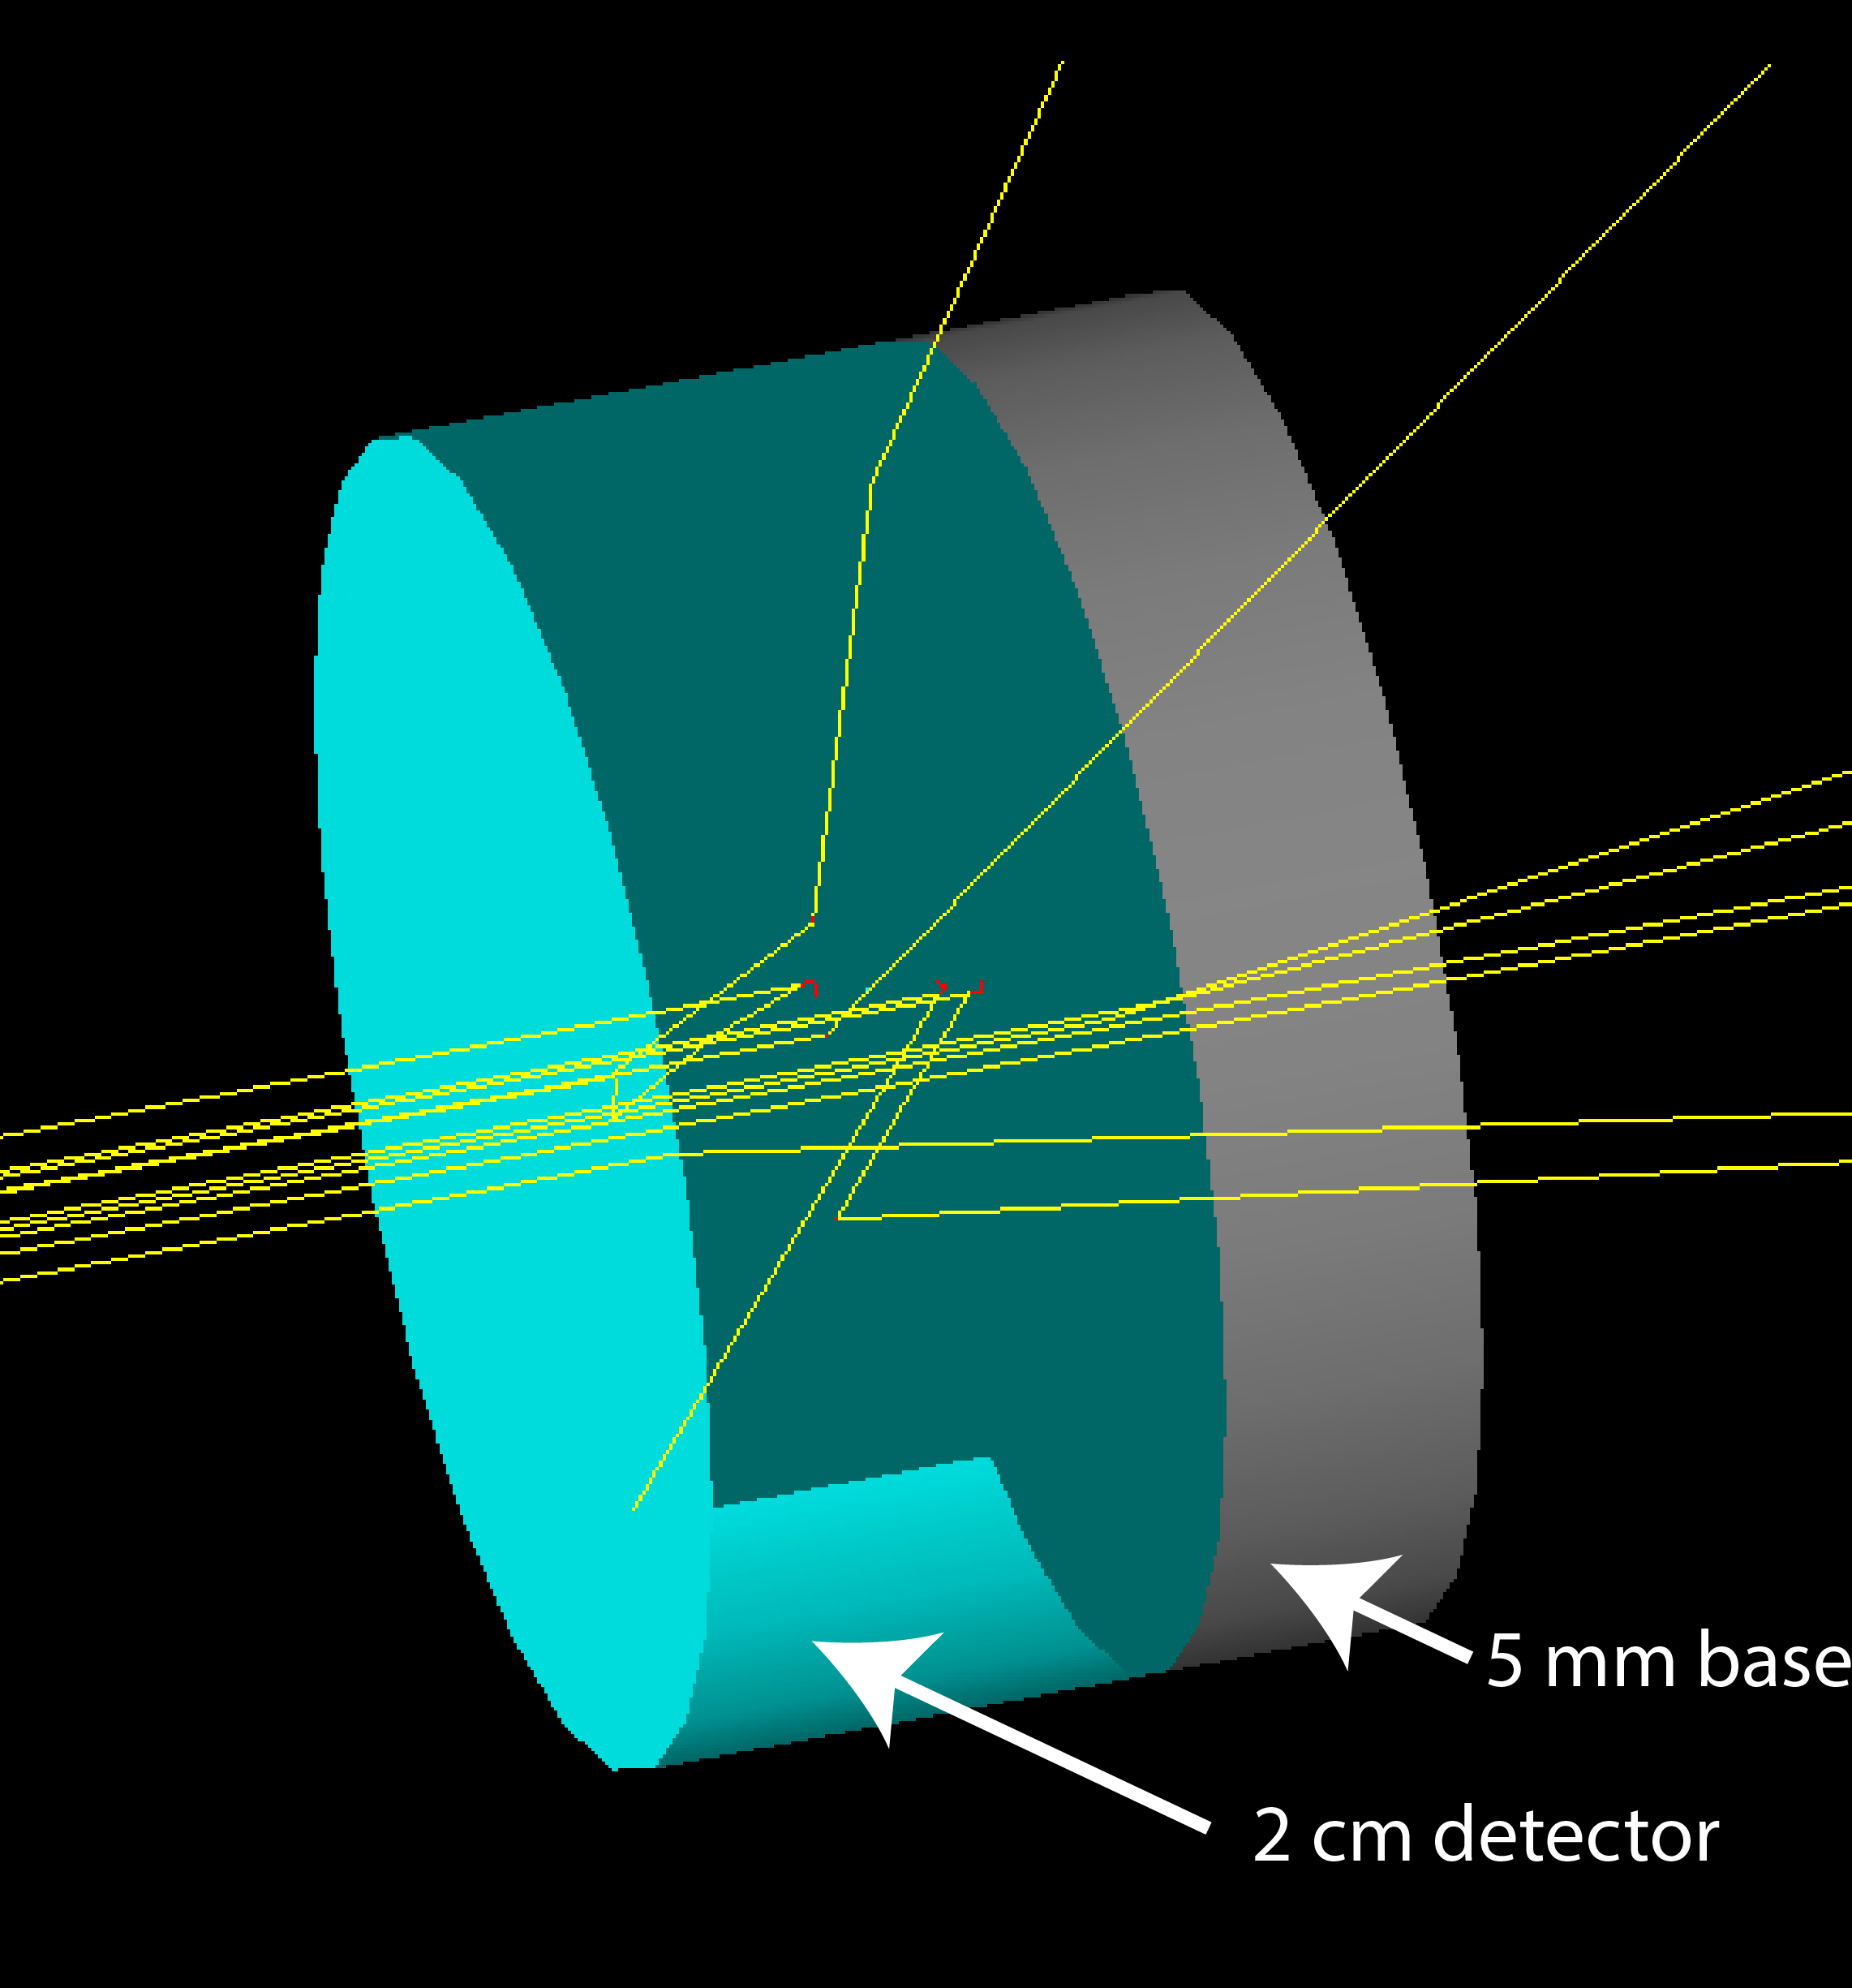
\includegraphics[width=\textwidth]{GEANT4AnnotatedGeo_EnergyDepEvent}
	\caption[GEANT4 Energy Depostion Geometry]{GEANT4 Geometry for the Simulation of Energy Deposition. What is shown are 10 photons from a \iso[60]{Co} source impigent upon a \SI{2}{\cm} thick detector.  The photon tracks are shown in yellow, while the electron tracks are shown in red.}
	\label{fig:EDepSimGeo}
\end{figure}
It is expected that the the Livermore data-driven parameterized electromagnetic physics will be necessary to calculate the ionizing energy deposition, extending the standard electro-magnetic physics down to \SI{1}{\kilo\eV}.
The neutron interactions will be simulated with a hadronic modules, using the \verb+HP+ flavored modules to use the ENDF cross sections to calculate the interaction rates.

It is proposed to validate the simulation by reproducing the single collision energy loss in water as well as comparing  the spectral shapes and averages of simulated and measured spectra.
The reproduction of the single collision energy loss will ensure that the electron physics are implemented correctly, while the simulation of the polymeric film energy deposition allows the user to gain confidence that the correct tracking and binning analysis has been implemented.
%%%%%%%%%%%%%%%%%%%%%%%%%%%%%%%%%%%%%%%%%%%%%%%%%%%%%%%%%%%%%%%%%%%%%%%%%%
%                                                      									 %
%                  		  	RPM Neutronic Performance   		            	 %
% 									                                                     %
%%%%%%%%%%%%%%%%%%%%%%%%%%%%%%%%%%%%%%%%%%%%%%%%%%%%%%%%%%%%%%%%%%%%%%%%%%
\section{RPM Neutronic Performance}
\label{sec:RPMNP}

Simulations are necessary to guide the design of a replacement RPM.
These simulations must provide a link between the measured performance of laboratory developed and characterized samples which are generally two inches and the performance of the film in an implemented detector system as it is prohibitive to construct and measure each film in an RPM.
Previous work showed that it is possible to adequately simulate detector performance in MCNPX, a Monte Carlo radiation transport code.
Generally these simulations involve correctly defining the simulation physics, source and geometry, and then using the correct tally measures to extract pertinent performance metrics.
After the simulation is completed is then benchmarked against measured quantities to provide a measure of confidence that the simulation provides an accurate model of reality.
Often (as in this case) the capability to directly measure the performance of the desired simulation geometry is not availabl is not available, and therefore the benchmarking must be completed on a comparable system on which it is possible to measure.

A validated simulation capability allows for one to explore the design space without having to physically build and test systems, which can be prohibitively expensive.
As a single film does not have the necessary interactions to fulfill the neutron count rate criteria multiple films are necessary, and the arrangement of these films provides a design space for a replacement RPM.
In the case of the RPM, there are several design parameters that can be explored:
\begin{itemize}
  \item the neutron absorber loading of the film,
  \item the thickness of the film,
  \item the geometry of the film (cylinders or sheets), and
  \item the placement of the films.
\end{itemize}
It is expected that the loading of the film will be limited by the optical clarity, and that the thickness of the film will be determined by the optimization of the energy deposition.
Thus, of the above design parameters only the geometric placement of the films is an available optimization space.

Preliminary work by this author provided a simple design in which the detector layers are linearly placed throughout the detector volume in an alternating fashion.
The analysis of the neutron flux throughout this detector lead to a flat flux profile as shown in \autoref{fig:AltLayerThermalNeutronFraction}.
\begin{figure}
  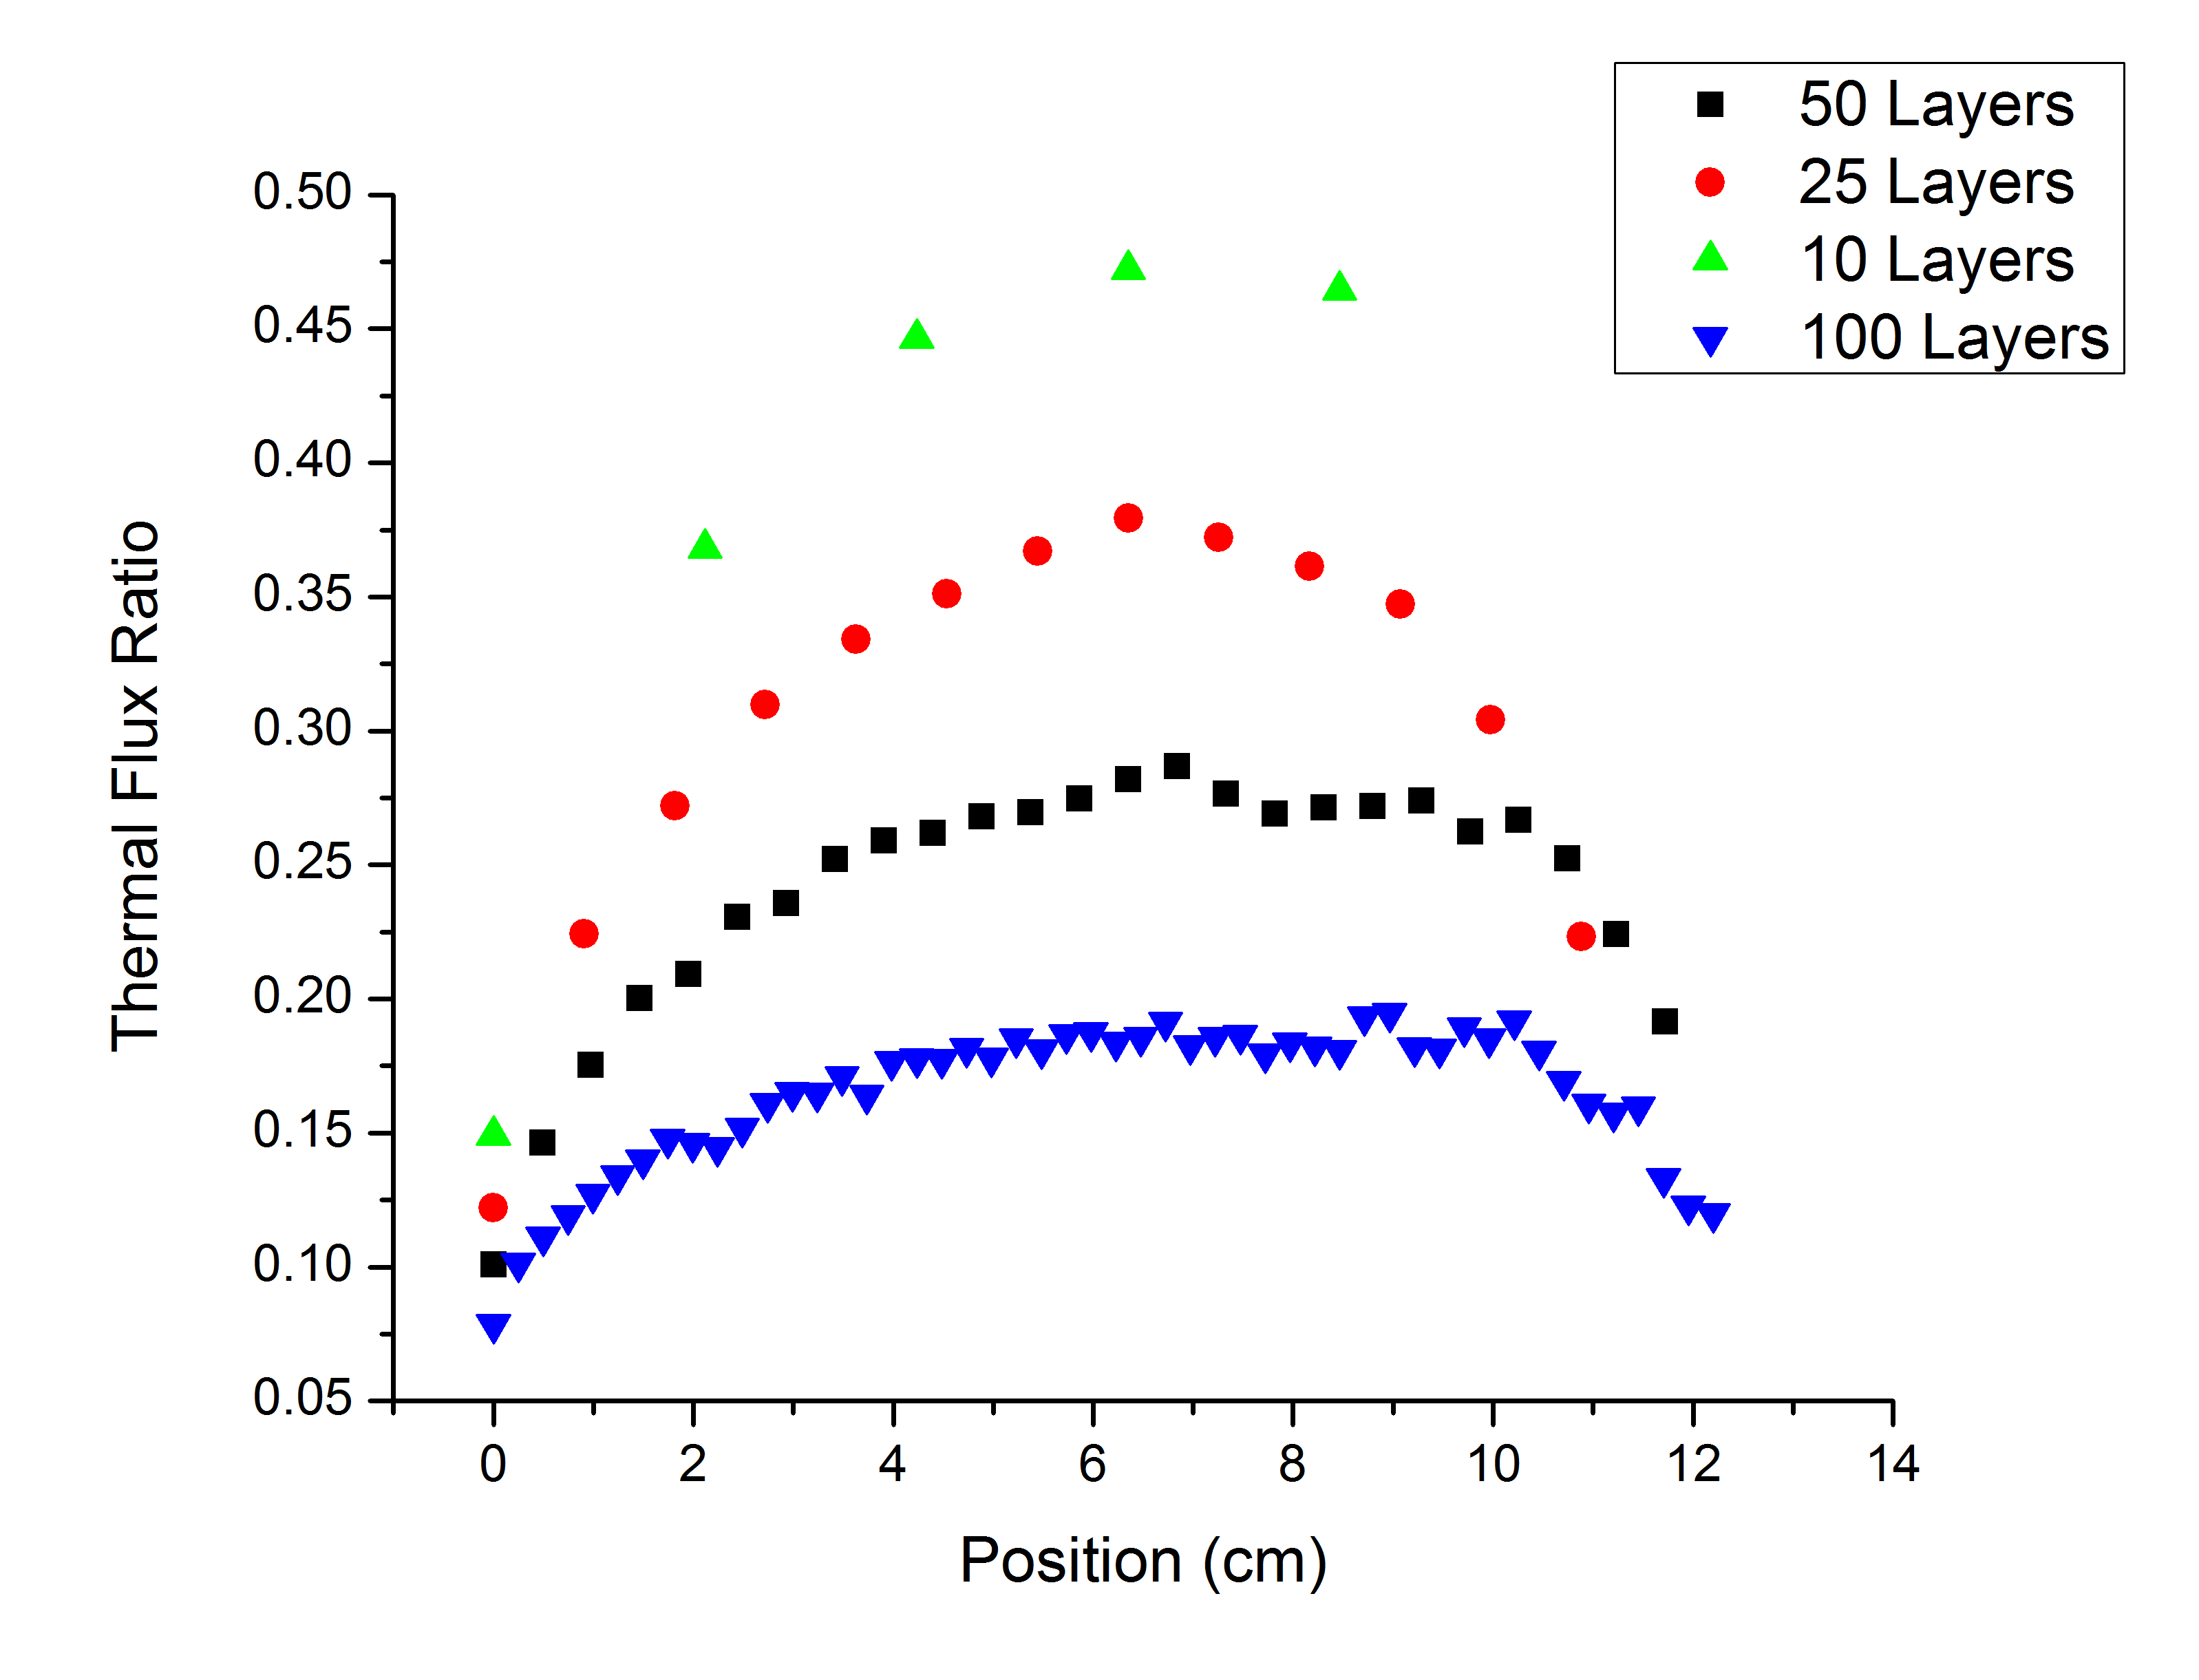
\includegraphics[width=\textwidth]{ThermalFluxRatioAltLayers}
	\caption{Fraction of the neutron flux that is thermalized through a alternating detector and moderator layered RPM.  The low thermal fluxes result in a poor utilization of the high thermal cross section of \iso[6]{Li}.}
	\label{fig:AltLayerThermalNeutronFraction}
\end{figure}
Several different strategies can then be used to optimize the geometry to ensure effective utilization of the thermal cross section of the absorber material.


\subsection{Proposed Work}
The cost of a radiation portal monitor can be broken into the material cost, the cost of the associated electronics, and the assembly cost.
The material cost consists of the neutron absorbing material, the cost of any neutron moderator materials, and the cost of any encasing material. 
It is thought that the \iso[6]{Li} will dominate the material cost.
As the detector is a scintillation based detector the electronics will consist of photomultiplier tubes and the associated electronics to create the necessary readout.
In addition there is also a cost to assemble the detector which will depend primarily on the number of components to assemble.

It is then proposed to design a methodology for the optimization of layered detectors that satisfy the criteria set forth in \autoref{tab:DHSCritera}.
The completed work will consist of a robust code base that can be easily adapted to different materials that can be easily optimized.
The utilization of this toolkit will yield a detector design that satisfies the DHS DNDO criteria while minimizing the mass of neutron absorber used in the detector.
\todo[inline]{It would be better if I could reformulate it to minimize the total cost of the detector - because in a carborane system it might not be the case that carborane scintillator dominates the detector cost}

\subsection{Methodology}
The proposed research laid out above will be accomplished using MCNPX to model the performance of a detector and genetic algorithms to search the possible candidate space of detector designs for the optimal design.
MCNPX was chosen as the neutronics simulation code because it is a well validated code that has been used by others to simulate RPM detector performance.
Previous experience has shown that the run time of the code is not that prohibitive (around \SI{1.72}{\minute}), but future enhancements might be to implement the geometry in a 1D transport code for significant speedup.
The MCNPX modeling is described in more detail in \autoref{sec:MCNPDetectorModelingMethod}
The optimization of the detector was chosen to be formulated as finding the detector design that maximizes the count rate per mass of absorber while still meeting the minimum count rate.
If the thickness of the RPM (\SI{12.7}{\cm}) is divided into equal slices where a slice can either contain a detector (\verb+1+) or moderator (\verb+0+) genetic algorithms can be used to effectively search this complex hypothesis space of possible detector designs for one that uses the minimum mass of absorber while still meeting the count rate criteria.
An overview to the genetic algorithm optimization is provided in \autoref{sec:GeneticAlgoSearchMethod}.
\subsubsection{MCNPX Detector Modeling}
\label{sec:MCNPDetectorModelingMethod}
The performance of films is simulated in MCNPX, a Monte Carlo transport code\cite{pelowitz_mcnpx_????}.
The geometry is as in the PNNL reports, namely a nano-gram of \iso[252]{Cf}  encased in \SI{0.5}{\cm} of lead and \SI{2.5}{\cm} of HDPE. 
The size of the RPM8 is \SI{12.7}{\cm} deep, by \SI{30}{\cm} wide and \SI{2}{\m} tall.

The interaction rate is calculated using the a cell flux tally in MCNPX and a tally multiplier card.
The tally multiplier card (FMn) is used to calculated any quantity of the form \eqref{eqn:FMCardForm} \cite{pelowitz_mcnpx_????}
\begin{align}
  \label{eqn:FMCardForm}
  I &= C\int\phi(E)\Re_m(E)dE
\end{align}
where \definevar{$I$}{Interaction rate}, \definevar{$\phi(E)$}{Energy dependent fluence} , \definevar{$\Re_m(E)$}{Response function operator} and $C$ is an arbitrary scalar for normalization.
An general example of the use of the FM card is shown in Listing \ref{lst:GeneralFMExample}, which is taken from the MCNPX manual \cite{pelowitz_mcnpx_????}.
% See pg. 4-41 of the MCNP manual
\begin{lstlisting}[caption={[Example usage of the FM card]Example usage of the FM card to calculate the number of reactions per \si{\cm\cubed} of type R in cell 8 of material M. The normalization is by atomic density, signified by the -1},label={lst:GeneralFMExample}]
F104: N 8
FM104 -1 M R
\end{lstlisting}

The reaction rate $\iso[6]{Li}\left(\text{n},\text{t}\right)\alpha$ can be calculated by then applying the appropriate input for the FMn card and using an F4 card to calculate $\phi(E)$.
It should be noted that depending on the form of the cell flux card it may be necessary to normalize by the volume of the cell, $\forall$.
\nomenclature{$\forall$}{Volume of the cell}

This is shown in Listing \ref{lst:InteractionRateRPM}, where the reaction number is 105 and the material number of the detector is 3.
The interaction rate in a simulated RPM8 replacement detector is calculated in a similar manner as the simulation of the measured detectors; the interaction rate as computed by the \verb+FMn+ is multiplied by the source strength and volume if necessary.
An example of the MCNPX input cards is shown in Listing \ref{lst:InteractionRateRPM}.
Given that there the thermal response is not desired, there is no need to subtract out the differences between the spectra, and the interaction rate is simply \eqref{eqn:RPM8InteractionRate}.
Note that in this calculation the source strength is set to be \SI{1}{\nano\gram} \iso[252]{Cf}, which has a neutron emission rate of \SI{2.3E3}{neutron\per\second}.
This is in accordance with the direct evaluation of the PNNL criteria, which require a absolute neutron count rate of \SI{2.5}{count\per\second\per\nano\gram\iso[252]{Cf}}.
\begin{lstlisting}[caption={[RPM8 ${}^{6}\text{Li}\left(\text{n},\text{t}\right)\alpha$ Reaction Rate]RPM8 ${}^{6}\text{Li}\left(\text{n},\text{t}\right)\alpha$ Reaction Rate. The detector is all of the layers of cell 500 inside universe 610. This tally is multiplied by an SD card to normalize by the volume},label={lst:InteractionRateRPM}]
FC4 (n,t) Reactions in Thin Film (Neutron Detector)
F4:n (500<610)
SD4 1
FM4 -1 3 105
\end{lstlisting}
\begin{align}
  \label{eqn:RPM8InteractionRate}
  I_{\text{sim}} &= S_0 I \\
  &= \SI{2.3E3}{neutron\per\second} I
\end{align}

$I_{\text{sim}}$ provides the total number of simulated neutron interactions in the detector.
However, not all of these interactions will lead to counts above the pulse height discriminator setting necessary for meeting the gamma intrinsic efficiency.
This is corrected for by scaling $I_{\text{sim}}$ by the fraction of counts, $\eta$, that occur above the gamma LLD \eqref{eqn:FractionOfCountsDefination}, \eqref{eqn:RPMCountRate}.
\begin{align}
  \label{eqn:FractionOfCountsDefination}
  \eta \equiv \frac{\int_{MLLD}^\infty p(x)dx}{\int_0^\infty p(x)dx}
\end{align}
\nomenclature{$p(x)$}{Measured spectra, as a function of channel number}
\begin{align}
 \label{eqn:RPMCountRate}
 \text{Count Rate} &= I_{\text{sim}} \eta
\end{align}

\subsubsection{Genetic Algorithm Search}
\label{sec:GeneticAlgoSearchMethod}
Genetic algorithms provide a search method analogous to biological evaluation. 
Rather than following a gradient of a response function, genetic algorithms generate possible hypothesis by repeatedly applying genetic operators (mutation and recombination) to the best currently known hypothesis for the generation of subsequent populations of hypothesis. 
In this way the search space of candidate hypothesis (possible detector designs) is searched to identify the best hypothesis; the design that uses the least amount of \iso[6]{Li} while meeting the criteria. 
The genetic algorithm typically consist of four tasks: 
\begin{enumerate}
  \item creating an initial population, 
  \item evaluating that populations fitness, 
  \item selecting members of the current population to breed, and 
  \item applying genetic operators to the selected members to breed the new population. 
\end{enumerate}	
This is completed until either a maximum generation is reached or the desired fitness is achieved.
\begin{figure}
\begin{algorithmic}
  \WHILE{$error>goal$}
		\FORALL{$p \in P$}
			\STATE{Compute fitness}
		\ENDFOR
		\FORALL{$p \in P$}	
			\STATE{Choose individuals based on fitness}
			\STATE{Select individuals for next population}
			\STATE{Crossover selected individuals}
			\STATE{Mutate selected individual}
		\ENDFOR
	\ENDWHILE
\end{algorithmic}
\caption{Genetic Program Outline}
\label{AlgoOutline}
\end{figure}

PyEvolve is a free Python implementation of genetic algorithms.
The PyEvolve toolkit was chosen for this work because of pythons scripting ability as well as the visualization and performance indicators of the PyEvolve toolkit.
In order to decrease the computational time is it proposed to use memoization to store detector solutions, where the bit string representation of the geometry is used as a hash for a dictionary.  
In addition, where possible multi-threading will be utilized.

%%%%%%%%%%%%%%%%%%%%%%%%%%%%%%%%%%%%%%%%%%%%%%%%%%%%%%%%%%%%%%%%%%%%%%%%%%
%                                                      									 %
%                  		  	RPM Light Collection                           %
% 									                                                     %
%%%%%%%%%%%%%%%%%%%%%%%%%%%%%%%%%%%%%%%%%%%%%%%%%%%%%%%%%%%%%%%%%%%%%%%%%%
\section{RPM Light Collection Performance}
\label{sec:RPMLCP}

There is no assurance that the detectors designed based on interaction rate would be feasible to construct; due to their low light output and opaqueness collecting the light from scintillation events would be extremely difficult.  
Additional simulation work then needs to be completed to ensure that a RPM in the layered detector design has a realistic method of collecting the light emitted from the scintillation events.
Light transport modeling provides a way to calculate the performance of such a design while providing insights for the improvement of a detector design.

Several previous authors have used the GEANT4 toolkit to simulate the light collection efficiency of their detector designs.
In PNNL 14283 the authors looked at a variety of different PMT placement and detectors designs to increase the light output of a detector in the Advanced Large-Area Plastic Scintillators (ALPS) project \cite{pnnl_14283}.
The authors found that for a \SI{127}{\cm} by \SI{57}{\cm} by \SI{5}{\cm} slab of BC-408 wrapped in a loose foil of 85\% reflectivity that the light output could be almost doubled by doubling the number of PMT's.
These results are summarized in \autoref{tab:PNNLLightCollectionEfficiency}.
\begin{table}
  \centering
  \caption[PNNL Light Collection Efficiencies]{Light collection efficiencies of several detector designs simulated by PNNL\cite{pnnl_14283}.}
  \label{tab:PNNLLightCollectionEfficiency}
  \begin{tabular}{c|c c}
  \toprule
  & \multicolumn{2}{c}{Light Collection Efficiency} \\
  Number of PMTs  & 2-in PMT & 5-in PMT \\
  \midrule
  2 & 7.0\% & 18.8\% \\
  4 & 13.3\% & 30.7\ \\
  6 & 18.4\% & 40.2\% \\
  \bottomrule
  \end{tabular}
\end{table}
In addition, other authors have reported on the simulation performance of a light guides and photon attenuation using the GEANT4 toolkit.
An overview of the light transport and scintillation processes available in GEANT4 is presented in \cite{riggi_introducing_2011}.
The authors also simulated a \SI{1}{\m} by \SI{1}{\cm} by \SI{1}{\cm} plastic strip in order to calculate the photon attenuation in the plastic.
Two orders of magnitude drop in the number of photons was calculated for photons collected \SI{90}{\cm} from the distance of emission, and was highly dependent of the reflectivity of the material encasing the plastic strip\cite{riggi_introducing_2011}.
Polymeric detectors containing PPO/POPOP as the fluor have also been modeled for the light transport with GEANT4\cite{5485130}.
This provides a measure of confidence that the films fabricated at the University of Tennessee containing PPO/POPOP can also be simulated without undo burden in finding light transport properties.

\subsection{Proposed Work}
It is proposed to simulate the neutronics, energy deposition, and light transport and collection of the optical photons with the GEANT4 toolkit to ensure that the proposed detector designs will be feasible. 
This will then have two parts:
\begin{enumerate}
  \item the fabrication and simulation of detectors whose performance can be measured in the laboratory, and
  \item the simulation of a RPM in the geometry specified by the neutronics calculations.
\end{enumerate}
It is also proposed to explore the design space of the light collection instrumentation, where such design options include
\begin{itemize}
  \item the use of a wavelength shifter (WLS) to increase the detected optical photons by decrease the optical photons absorbed in the light guide,
  \item the design of a light guide to enhance the photons reflected towards the PMT,
  \item the application of different light reflection techniques (air gap, Teflon tape, aluminized mylar) to enhance the light collection, and
  \item the placement of PMT's for their effective utilization.
\end{itemize}
The developed GEANT4 application will then have the ability to fully simulate the performance of a replacement RPM.

\subsection{Methodology}
The full simulation of the light transport of the RPM will be completed in with the GEANT4 toolkit.
GEANT4 offers three example simulations for generation and tracking of optical photons (\verb+ExampleN06+, \verb+extended/LXe+, and \verb+extended/WLS+).
These examples will be adapted for the purposes of this simulation.
However, it should be noted that the \verb+LXe+ and \verb+WLS+ utilize a sensitive detector which kills tracks, and for the purposes of the simulation of the RPM this will not be implemented.

The validation of the GEANT4 simulations will be completed with the fabrication of a 4 inches by 6 inches layered detector to allow the toolset to be benchmarked against measurements.
Detectors of various materials (boron loaded plastic, lithium loaded polymers, and LiF/ZnS(Ag)) will be tested to avoid a basis in the simulation parameters.
Where possible, the optical parameters of the materials will be taken from the literature.
However, it they cannot be found a similar material for which the property is know will be substituted.
In addition, rather than providing reflectivity parameters for each material, a model of optical surface will be used according to the work of Janecek\cite{5485130}. 

The GEANT4 light transport simulation code base will be written such that bit-string geometries from genetic algorithm optimization can be directly implemented.
With this formulation it will be possible to reuse the genetic algorithm optimization code base, while additionally providing a validation of the GEANT4 neutronic calculations against the MCNPX.
